La derivata di Caputo è approssimata con la formula L1 sulla griglia temporale $0=t_0<t_1<\cdots<t_M=T$, dove $M$ indica il numero di sottointervalli temporali:
\begin{equation}
\begin{aligned}
\CD{\gamma}u(t_n)&\approx\frac{1}{\Gamma(2-\gamma)}\sum_{k=1}^n
\frac{u^k-u^{k-1}}{\Delta t_k}\\
&\quad\times\left[(t_n-t_{k-1})^{1-\gamma}-(t_n-t_k)^{1-\gamma}\right],\\[-1pt]
&\hspace{7em}n=1,\ldots,M.
\end{aligned}
\label{eq:l1}
\end{equation}
Si usa $\gamma=\beta$ nella matrice e $\gamma=\alpha$ nel tracciante. I pesi sono calcolati usando i passi effettivi anche quando la griglia è non uniforme \citep{kopteva2019error}. Nello studio spaziale si usano elementi $Q_2/Q_1/Q_1$ per spostamento, pressione e tracciante; nello studio temporale la discretizzazione spaziale è $Q_2/Q_2/Q_2$ per ridurre la contaminazione spaziale.

\subsection{Verifica mediante soluzioni manufatte}

Sul quadrato $\Omega=(0,1)^2$ si prescrivono
\begin{align*}
\mathbf d^*(x,y,t)&=t^2\begin{pmatrix}\sin(\pi x)\sin(\pi y)\\\sin(2\pi x)\sin(\pi y)\end{pmatrix},\\
p^*(x,y,t)&=t^2\cos(\pi x)\cos(\pi y),\\
c^*(x,y,t)&=1+\delta t^2\cos(\pi x)\cos(\pi y),\quad 0<\delta<1,
\end{align*}
con $\mathbf q^*=-\mathbb K_h\nabla p^*$. I termini sorgente sono derivati analiticamente dalle equazioni indipendentemente dal codice del solutore. Si usa $\CD{\gamma}t^2=\Gamma(3)t^{2-\gamma}/\Gamma(3-\gamma)$ per calcolare i contributi frazionari. I dati iniziali indotti dalle soluzioni manufatte sono $\mathbf d^*(\cdot,0)=0$, $p^*(\cdot,0)=0$ e $c^*(\cdot,0)=1$; le condizioni al contorno sono ricavate dalle stesse funzioni esatte. Gli errori sono misurati in $L^2$ e $H^1$ sui tre campi.

\subsection{Caso anatomico 2D}

Il caso è il soggetto \texttt{BraTS20\_Training\_001} del benchmark BraTS 2020. Le modalità T1, T1ce, T2 e FLAIR e la segmentazione sono caricate dai volumi NIfTI, orientate in RAS+ e controllate per corrispondenza di griglia. La sezione assiale $k=67$ è selezionata automaticamente come sezione con massima estensione tumorale. BraTS fornisce label 1 (core necrotico/non-enhancing), 2 (edema) e 4 (enhancing tumor); esse non costituiscono una segmentazione della sostanza bianca \citep{menze2015the,bakas2017advancing,bakas2018identifying}.

Il dominio computazionale è un \emph{brain-parenchyma proxy} ricavato dal supporto dell'immagine, non una segmentazione indipendente della sostanza bianca. La mesh quadrilatera di riferimento ha dimensione di lato obiettivo 3 mm, 1901 elementi e 2003 nodi. Le scale sono $L_0=10$ mm, $T_0=100$ s, $E_0=1000$ Pa e $c_{\rm ref}=1$ mol m$^{-3}$. I coefficienti adimensionali fissi sono $\nu=0.35$, $b=0.8$, $S_p=0.5$, $K_h=0.2$, $\eta_v=0.45$, $\tau_v=1$ e $\phi_0=0.2$, in deformazione piana. Il vettore di riferimento è $\tht^\dagger=(0.70,0.45,0.08,2.5)$, equivalente a $D_{\rm phys}=8\times10^{-8}$ m$^2$/s ed $E_{\rm phys}=2500$ Pa.

Le forzanti sono sintetiche: il tracciante iniziale è una gaussiana di baseline 0.1, ampiezza 1 e larghezza 8 mm; la sorgente fluida ha ampiezza 0.6, larghezza 9 mm e decadimento esponenziale; la forza meccanica ha ampiezze $(0.8,0.6)$, larghezza 12 mm e profilo sinusoidale di pulsazione adimensionale $\pi$. I centri sono collocati sul centroide della lesione, con distanza dal centroide pari a zero per costruzione. Il contorno esterno è vincolato con $\mathbf d=0$; le condizioni di non-flusso per Darcy e per il flusso totale del tracciante sono applicate su tutte le frontiere. Sono ipotesi di scenario, non forzanti fisiologiche misurate.

\begin{figure*}[t]
\centering
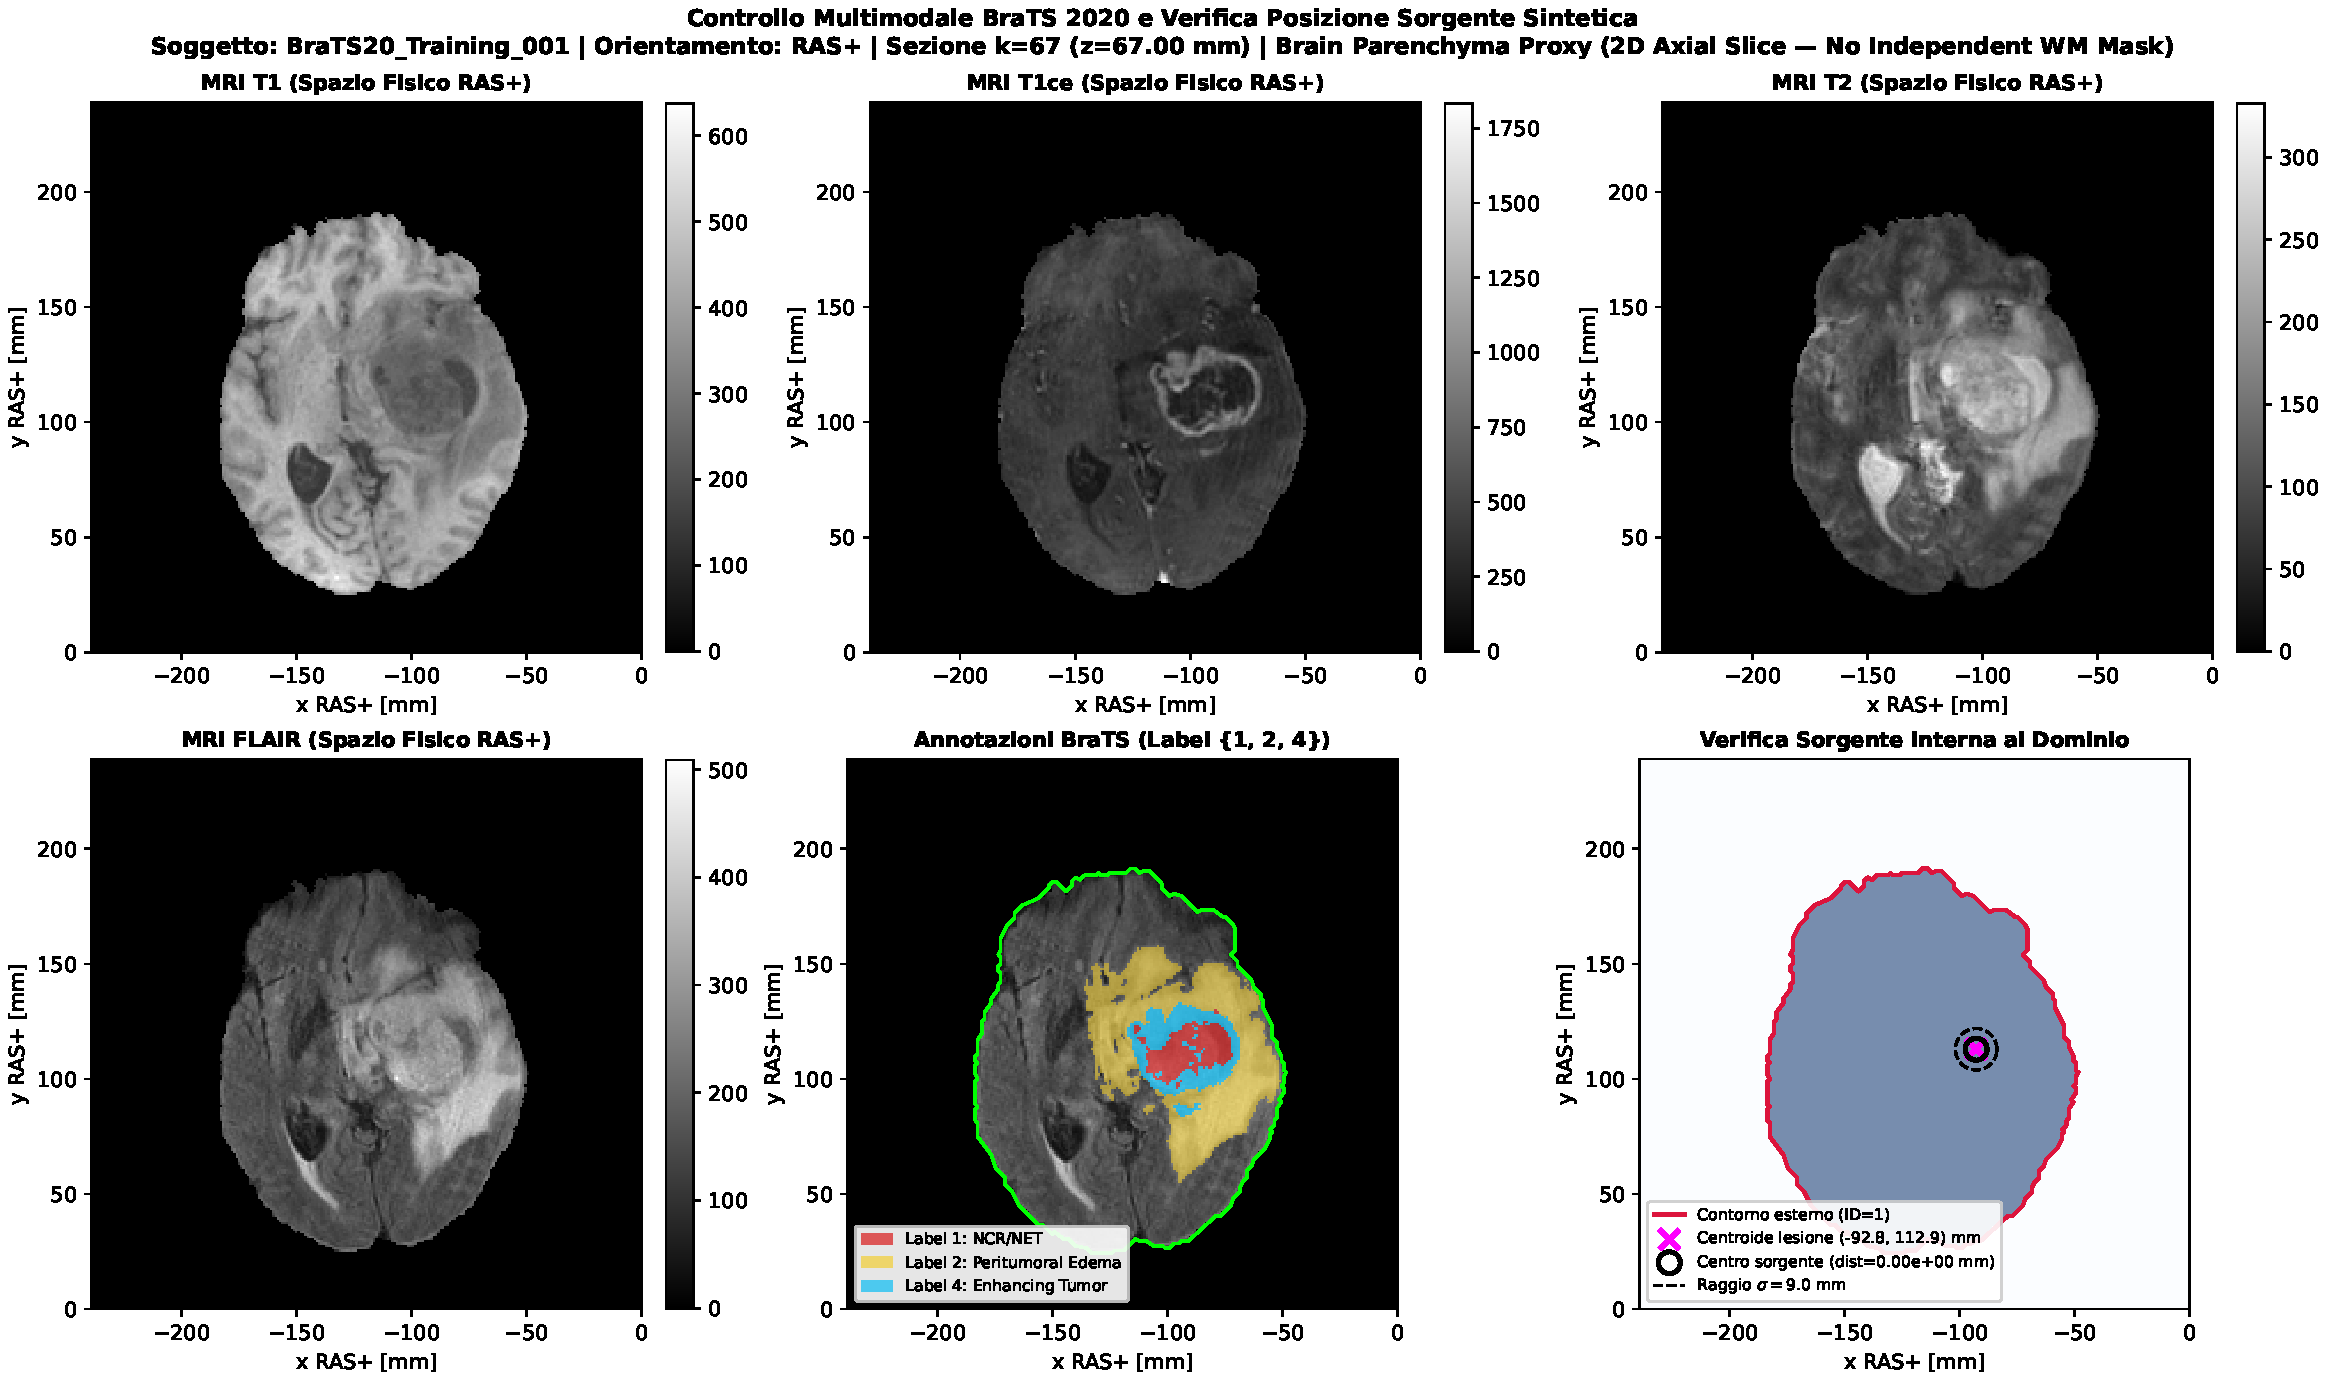
\includegraphics[width=0.94\textwidth]{paper/fig01_multimodal_anatomy_and_annotations.pdf}
\caption{Quattro modalità MRI e annotazioni del caso BraTS selezionato. L'immagine fornisce anatomia statica e localizzazione della lesione; non contiene le traiettorie temporali simulate dal modello.}
\label{fig:anatomy}
\end{figure*}

\begin{figure*}[t]
\centering
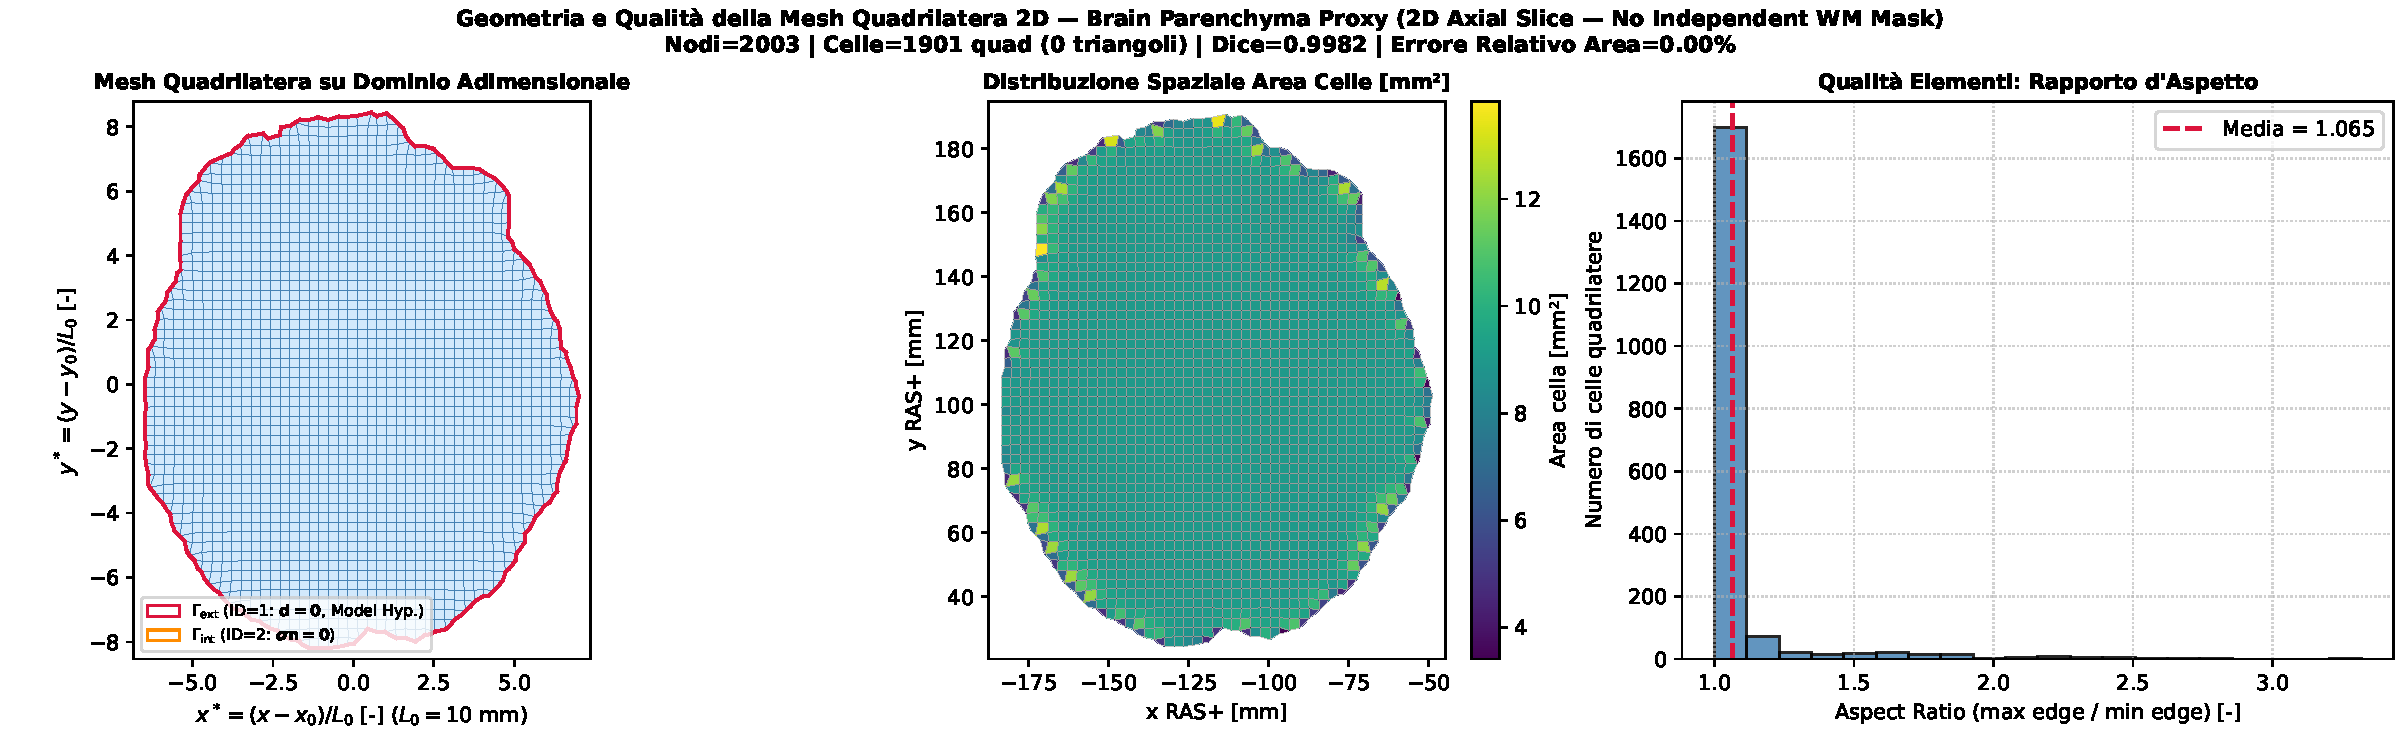
\includegraphics[width=0.94\textwidth]{paper/fig02_anatomical_mask_and_quad_mesh_quality.pdf}
\caption{Dominio proxy e mesh quadrilatera. Le metriche valutano l'approssimazione della maschera scelta, non l'accuratezza istologica o la segmentazione della sostanza bianca.}
\label{fig:mesh}
\end{figure*}

\subsection{Identificabilità e twin experiments sintetici}

L'esperimento di identificabilità usa soltanto osservazioni del tracciante: una griglia spaziale $6\times6$ e cinque istanti adimensionali $t\in\{0.15,0.30,0.50,0.75,1.0\}$, per un totale di $N_{\rm obs}=180$ osservazioni. La discretizzazione inversa di riferimento è $N=16$, $M=80$, $T=1$ e griglia temporale graduata con esponente $r=1.5$, con elementi $Q_2/Q_1/Q_1$. I limiti sono $\alpha,\beta\in[0.15,0.9]$, $D\in[0.01,0.5]$ ed $E\in[0.5,6]$. Il Jacobiano è calcolato con differenze finite centrate nelle coordinate normalizzate, usando passo $10^{-4}$ e pesi identità per le osservazioni adimensionali, in assenza di una covarianza empirica clinica.

Per i twin experiments, il vettore obiettivo è generato sulla discretizzazione $N=32$, $M=160$ e osservato tramite lo stesso insieme di 180 misure; l'inversione di riferimento usa $N=16$, $M=80$. Campo iniziale e callback delle forzanti sono mantenuti identici tra target e inverso, a meno della valutazione sulle rispettive discretizzazioni. Il vettore obiettivo pulito è congelato e identificato dall'hash SHA-256 riportato nell'Appendice~\ref{app:repro}. La campagna senza rumore riutilizza tre run CPSO con budget pianificato di 600 valutazioni del problema diretto. La campagna rumorosa comprende cinque realizzazioni indipendenti per ciascuno dei livelli nominali $\eta\in\{0.05,0.10\}$; per tutte e dieci le run rumorose il seed dell'ottimizzatore è mantenuto fisso, in modo da isolare descrittivamente l'effetto delle realizzazioni del rumore condizionatamente alla medesima configurazione iniziale dello sciame. I seed dei dati rumorosi sono distinti e registrati negli artefatti supplementari.

Nella campagna finale CPSO usa 10 particelle, fino a 60 iterazioni e un budget pianificato di 600 valutazioni FEM per run. Per $\eta=0$ è utilizzata la pesatura deterministica (Mode A) con $\lambda_A=10^{-4}$. Per i casi rumorosi è utilizzata la pesatura con covarianza inversa esatta (Mode B covariance), con $\sigma=\eta\|\mathbf y_{\rm clean}\|_\infty$ e $\lambda_B=7.2$, convertito dalla scala di riferimento $\eta_{\rm ref}=0.05$ secondo $\lambda_B^{\rm eq}(\eta)=N_{\rm obs}\lambda_A/\eta^2$. La scelta mantiene $\lambda_B=7.2$ anche per $\eta=0.10$, per cui non conserva il medesimo rapporto fra dati e penalizzazione nei due livelli: il valore equivalente a $\eta=0.10$ sarebbe $1.8$. Di conseguenza, il confronto tra i due livelli descrive il protocollo effettivamente eseguito e non isola l'effetto del rumore da quello del bilanciamento del funzionale. Il controllo di normalizzazione e di isolamento del target pulito è riportato nell'Appendice~\ref{app:objective}. Il rapporto realizzato $\|\boldsymbol\epsilon\|_2/\|\mathbf y_{\rm clean}\|_2$ è riportato separatamente dal livello nominale, poiché i due valori non coincidono in generale.

Il budget di 600 valutazioni è un limite computazionale, non un criterio di convergenza. Le run finali riportate hanno esaurito il budget e le stime sono pertanto i migliori candidati individuati nelle rispettive storie, non minimi locali o globali certificati. Inoltre, mantenendo fisso il seed CPSO nella campagna rumorosa, la dispersione osservata descrive la sensibilità al rumore per una singola configurazione dell'ottimizzatore, non la variabilità complessiva che deriverebbe anche da seed CPSO indipendenti.

\subsection{Definizione della pesatura obiettivo}

Il confronto dei modi di pesatura valuta tre convenzioni per il residuo $\mathbf r=\mathcal G_h(\boldsymbol\theta)-\mathbf y$: (A) $W_A=I/(\sqrt{N_{\rm obs}}s_{\rm ref})$; (B-mean) $W_{B,\rm mean}=I/(\sqrt{N_{\rm obs}}\sigma)$; (B-cov) $W_{B,\rm cov}=I/\sigma$, con $s_{\rm ref}=\|\mathbf y_{\rm clean}\|_\infty$ e $\sigma=\eta s_{\rm ref}$. Ne segue, a parità di residuo, $J_{\rm data}^{B,\rm mean}/J_{\rm data}^{A}=\eta^{-2}$ e $J_{\rm data}^{B,\rm cov}/J_{\rm data}^{A}=N_{\rm obs}/\eta^2$. I modi non sono intercambiabili mantenendo fisso $\lambda$. L'analisi è un confronto della scala del funzionale su candidati già disponibili, non una nuova ottimizzazione né una regola automatica per calibrare $\lambda$.
